% !TEX encoding = UTF-8 Unicode
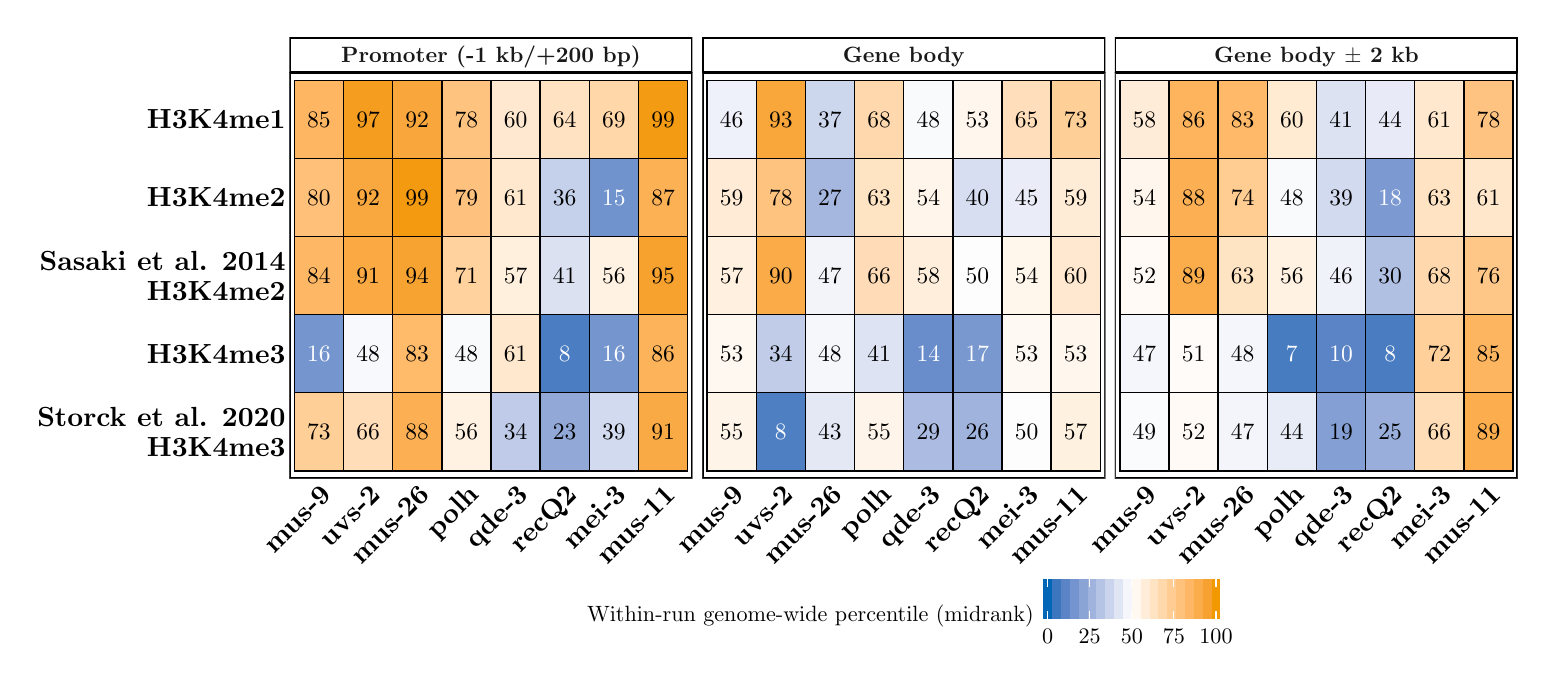
\begin{tikzpicture}[x=1pt,y=1pt]
\definecolor{fillColor}{RGB}{255,255,255}
\path[use as bounding box,fill=fillColor,fill opacity=0.00] (0,0) rectangle (542.02,231.26);
\begin{scope}
\path[clip] (  0.00,  0.00) rectangle (542.02,231.26);
\definecolor{drawColor}{RGB}{255,255,255}
\definecolor{fillColor}{RGB}{255,255,255}

\path[draw=drawColor,line width= 0.7pt,line join=round,line cap=round,fill=fillColor] ( -0.00,  0.00) rectangle (542.02,231.26);
\end{scope}
\begin{scope}
\path[clip] ( 94.59, 68.29) rectangle (240.23,215.09);
\definecolor{drawColor}{RGB}{0,0,0}
\definecolor{fillColor}{RGB}{255,255,255}

\path[draw=drawColor,line width= 1.1pt,line join=round,line cap=round,fill=fillColor] ( 94.59, 68.29) rectangle (240.23,215.09);
\definecolor{fillColor}{RGB}{254,182,98}

\path[draw=drawColor,line width= 0.5pt,fill=fillColor] ( 96.36,184.03) rectangle (114.12,212.26);
\definecolor{fillColor}{RGB}{245,157,30}

\path[draw=drawColor,line width= 0.5pt,fill=fillColor] (114.12,184.03) rectangle (131.89,212.26);
\definecolor{fillColor}{RGB}{249,167,61}

\path[draw=drawColor,line width= 0.5pt,fill=fillColor] (131.89,184.03) rectangle (149.65,212.26);
\definecolor{fillColor}{RGB}{255,195,128}

\path[draw=drawColor,line width= 0.5pt,fill=fillColor] (149.65,184.03) rectangle (167.41,212.26);
\definecolor{fillColor}{RGB}{255,232,207}

\path[draw=drawColor,line width= 0.5pt,fill=fillColor] (167.41,184.03) rectangle (185.17,212.26);
\definecolor{fillColor}{RGB}{255,226,193}

\path[draw=drawColor,line width= 0.5pt,fill=fillColor] (185.17,184.03) rectangle (202.93,212.26);
\definecolor{fillColor}{RGB}{255,215,169}

\path[draw=drawColor,line width= 0.5pt,fill=fillColor] (202.93,184.03) rectangle (220.69,212.26);
\definecolor{fillColor}{RGB}{243,155,19}

\path[draw=drawColor,line width= 0.5pt,fill=fillColor] (220.69,184.03) rectangle (238.46,212.26);
\definecolor{fillColor}{RGB}{255,192,121}

\path[draw=drawColor,line width= 0.5pt,fill=fillColor] ( 96.36,155.80) rectangle (114.12,184.03);
\definecolor{fillColor}{RGB}{249,168,63}

\path[draw=drawColor,line width= 0.5pt,fill=fillColor] (114.12,155.80) rectangle (131.89,184.03);
\definecolor{fillColor}{RGB}{243,154,16}

\path[draw=drawColor,line width= 0.5pt,fill=fillColor] (131.89,155.80) rectangle (149.65,184.03);
\definecolor{fillColor}{RGB}{255,194,126}

\path[draw=drawColor,line width= 0.5pt,fill=fillColor] (149.65,155.80) rectangle (167.41,184.03);
\definecolor{fillColor}{RGB}{255,232,205}

\path[draw=drawColor,line width= 0.5pt,fill=fillColor] (167.41,155.80) rectangle (185.17,184.03);
\definecolor{fillColor}{RGB}{197,208,234}

\path[draw=drawColor,line width= 0.5pt,fill=fillColor] (185.17,155.80) rectangle (202.93,184.03);
\definecolor{fillColor}{RGB}{113,147,205}

\path[draw=drawColor,line width= 0.5pt,fill=fillColor] (202.93,155.80) rectangle (220.69,184.03);
\definecolor{fillColor}{RGB}{252,177,85}

\path[draw=drawColor,line width= 0.5pt,fill=fillColor] (220.69,155.80) rectangle (238.46,184.03);
\definecolor{fillColor}{RGB}{254,183,100}

\path[draw=drawColor,line width= 0.5pt,fill=fillColor] ( 96.36,127.57) rectangle (114.12,155.80);
\definecolor{fillColor}{RGB}{250,169,67}

\path[draw=drawColor,line width= 0.5pt,fill=fillColor] (114.12,127.57) rectangle (131.89,155.80);
\definecolor{fillColor}{RGB}{247,163,50}

\path[draw=drawColor,line width= 0.5pt,fill=fillColor] (131.89,127.57) rectangle (149.65,155.80);
\definecolor{fillColor}{RGB}{255,210,158}

\path[draw=drawColor,line width= 0.5pt,fill=fillColor] (149.65,127.57) rectangle (167.41,155.80);
\definecolor{fillColor}{RGB}{255,239,221}

\path[draw=drawColor,line width= 0.5pt,fill=fillColor] (167.41,127.57) rectangle (185.17,155.80);
\definecolor{fillColor}{RGB}{219,225,241}

\path[draw=drawColor,line width= 0.5pt,fill=fillColor] (185.17,127.57) rectangle (202.93,155.80);
\definecolor{fillColor}{RGB}{255,242,227}

\path[draw=drawColor,line width= 0.5pt,fill=fillColor] (202.93,127.57) rectangle (220.69,155.80);
\definecolor{fillColor}{RGB}{247,162,47}

\path[draw=drawColor,line width= 0.5pt,fill=fillColor] (220.69,127.57) rectangle (238.46,155.80);
\definecolor{fillColor}{RGB}{116,149,206}

\path[draw=drawColor,line width= 0.5pt,fill=fillColor] ( 96.36, 99.34) rectangle (114.12,127.57);
\definecolor{fillColor}{RGB}{248,249,252}

\path[draw=drawColor,line width= 0.5pt,fill=fillColor] (114.12, 99.34) rectangle (131.89,127.57);
\definecolor{fillColor}{RGB}{255,186,106}

\path[draw=drawColor,line width= 0.5pt,fill=fillColor] (131.89, 99.34) rectangle (149.65,127.57);
\definecolor{fillColor}{RGB}{249,250,252}

\path[draw=drawColor,line width= 0.5pt,fill=fillColor] (149.65, 99.34) rectangle (167.41,127.57);
\definecolor{fillColor}{RGB}{255,232,206}

\path[draw=drawColor,line width= 0.5pt,fill=fillColor] (167.41, 99.34) rectangle (185.17,127.57);
\definecolor{fillColor}{RGB}{75,125,194}

\path[draw=drawColor,line width= 0.5pt,fill=fillColor] (185.17, 99.34) rectangle (202.93,127.57);
\definecolor{fillColor}{RGB}{117,149,206}

\path[draw=drawColor,line width= 0.5pt,fill=fillColor] (202.93, 99.34) rectangle (220.69,127.57);
\definecolor{fillColor}{RGB}{253,179,90}

\path[draw=drawColor,line width= 0.5pt,fill=fillColor] (220.69, 99.34) rectangle (238.46,127.57);
\definecolor{fillColor}{RGB}{255,207,152}

\path[draw=drawColor,line width= 0.5pt,fill=fillColor] ( 96.36, 71.11) rectangle (114.12, 99.34);
\definecolor{fillColor}{RGB}{255,221,184}

\path[draw=drawColor,line width= 0.5pt,fill=fillColor] (114.12, 71.11) rectangle (131.89, 99.34);
\definecolor{fillColor}{RGB}{252,176,83}

\path[draw=drawColor,line width= 0.5pt,fill=fillColor] (131.89, 71.11) rectangle (149.65, 99.34);
\definecolor{fillColor}{RGB}{255,242,227}

\path[draw=drawColor,line width= 0.5pt,fill=fillColor] (149.65, 71.11) rectangle (167.41, 99.34);
\definecolor{fillColor}{RGB}{191,203,232}

\path[draw=drawColor,line width= 0.5pt,fill=fillColor] (167.41, 71.11) rectangle (185.17, 99.34);
\definecolor{fillColor}{RGB}{146,169,216}

\path[draw=drawColor,line width= 0.5pt,fill=fillColor] (185.17, 71.11) rectangle (202.93, 99.34);
\definecolor{fillColor}{RGB}{209,218,238}

\path[draw=drawColor,line width= 0.5pt,fill=fillColor] (202.93, 71.11) rectangle (220.69, 99.34);
\definecolor{fillColor}{RGB}{250,170,68}

\path[draw=drawColor,line width= 0.5pt,fill=fillColor] (220.69, 71.11) rectangle (238.46, 99.34);

\node[text=drawColor,anchor=base,inner sep=0pt, outer sep=0pt, scale=  0.85] at (105.24,195.21) {85};

\node[text=drawColor,anchor=base,inner sep=0pt, outer sep=0pt, scale=  0.85] at (123.01,195.21) {97};

\node[text=drawColor,anchor=base,inner sep=0pt, outer sep=0pt, scale=  0.85] at (140.77,195.21) {92};

\node[text=drawColor,anchor=base,inner sep=0pt, outer sep=0pt, scale=  0.85] at (158.53,195.21) {78};

\node[text=drawColor,anchor=base,inner sep=0pt, outer sep=0pt, scale=  0.85] at (176.29,195.21) {60};

\node[text=drawColor,anchor=base,inner sep=0pt, outer sep=0pt, scale=  0.85] at (194.05,195.21) {64};

\node[text=drawColor,anchor=base,inner sep=0pt, outer sep=0pt, scale=  0.85] at (211.81,195.21) {69};

\node[text=drawColor,anchor=base,inner sep=0pt, outer sep=0pt, scale=  0.85] at (229.58,195.21) {99};

\node[text=drawColor,anchor=base,inner sep=0pt, outer sep=0pt, scale=  0.85] at (105.24,166.98) {80};

\node[text=drawColor,anchor=base,inner sep=0pt, outer sep=0pt, scale=  0.85] at (123.01,166.98) {92};

\node[text=drawColor,anchor=base,inner sep=0pt, outer sep=0pt, scale=  0.85] at (140.77,166.98) {99};

\node[text=drawColor,anchor=base,inner sep=0pt, outer sep=0pt, scale=  0.85] at (158.53,166.98) {79};

\node[text=drawColor,anchor=base,inner sep=0pt, outer sep=0pt, scale=  0.85] at (176.29,166.98) {61};

\node[text=drawColor,anchor=base,inner sep=0pt, outer sep=0pt, scale=  0.85] at (194.05,166.98) {36};
\definecolor{drawColor}{RGB}{255,255,255}

\node[text=drawColor,anchor=base,inner sep=0pt, outer sep=0pt, scale=  0.85] at (211.81,166.98) {15};
\definecolor{drawColor}{RGB}{0,0,0}

\node[text=drawColor,anchor=base,inner sep=0pt, outer sep=0pt, scale=  0.85] at (229.58,166.98) {87};

\node[text=drawColor,anchor=base,inner sep=0pt, outer sep=0pt, scale=  0.85] at (105.24,138.75) {84};

\node[text=drawColor,anchor=base,inner sep=0pt, outer sep=0pt, scale=  0.85] at (123.01,138.75) {91};

\node[text=drawColor,anchor=base,inner sep=0pt, outer sep=0pt, scale=  0.85] at (140.77,138.75) {94};

\node[text=drawColor,anchor=base,inner sep=0pt, outer sep=0pt, scale=  0.85] at (158.53,138.75) {71};

\node[text=drawColor,anchor=base,inner sep=0pt, outer sep=0pt, scale=  0.85] at (176.29,138.75) {57};

\node[text=drawColor,anchor=base,inner sep=0pt, outer sep=0pt, scale=  0.85] at (194.05,138.75) {41};

\node[text=drawColor,anchor=base,inner sep=0pt, outer sep=0pt, scale=  0.85] at (211.81,138.75) {56};

\node[text=drawColor,anchor=base,inner sep=0pt, outer sep=0pt, scale=  0.85] at (229.58,138.75) {95};
\definecolor{drawColor}{RGB}{255,255,255}

\node[text=drawColor,anchor=base,inner sep=0pt, outer sep=0pt, scale=  0.85] at (105.24,110.52) {16};
\definecolor{drawColor}{RGB}{0,0,0}

\node[text=drawColor,anchor=base,inner sep=0pt, outer sep=0pt, scale=  0.85] at (123.01,110.52) {48};

\node[text=drawColor,anchor=base,inner sep=0pt, outer sep=0pt, scale=  0.85] at (140.77,110.52) {83};

\node[text=drawColor,anchor=base,inner sep=0pt, outer sep=0pt, scale=  0.85] at (158.53,110.52) {48};

\node[text=drawColor,anchor=base,inner sep=0pt, outer sep=0pt, scale=  0.85] at (176.29,110.52) {61};
\definecolor{drawColor}{RGB}{255,255,255}

\node[text=drawColor,anchor=base,inner sep=0pt, outer sep=0pt, scale=  0.85] at (194.05,110.52) {8};

\node[text=drawColor,anchor=base,inner sep=0pt, outer sep=0pt, scale=  0.85] at (211.81,110.52) {16};
\definecolor{drawColor}{RGB}{0,0,0}

\node[text=drawColor,anchor=base,inner sep=0pt, outer sep=0pt, scale=  0.85] at (229.58,110.52) {86};

\node[text=drawColor,anchor=base,inner sep=0pt, outer sep=0pt, scale=  0.85] at (105.24, 82.28) {73};

\node[text=drawColor,anchor=base,inner sep=0pt, outer sep=0pt, scale=  0.85] at (123.01, 82.28) {66};

\node[text=drawColor,anchor=base,inner sep=0pt, outer sep=0pt, scale=  0.85] at (140.77, 82.28) {88};

\node[text=drawColor,anchor=base,inner sep=0pt, outer sep=0pt, scale=  0.85] at (158.53, 82.28) {56};

\node[text=drawColor,anchor=base,inner sep=0pt, outer sep=0pt, scale=  0.85] at (176.29, 82.28) {34};

\node[text=drawColor,anchor=base,inner sep=0pt, outer sep=0pt, scale=  0.85] at (194.05, 82.28) {23};

\node[text=drawColor,anchor=base,inner sep=0pt, outer sep=0pt, scale=  0.85] at (211.81, 82.28) {39};

\node[text=drawColor,anchor=base,inner sep=0pt, outer sep=0pt, scale=  0.85] at (229.58, 82.28) {91};
\definecolor{drawColor}{gray}{0.20}

\path[draw=drawColor,line width= 0.7pt,line join=round,line cap=round] ( 94.59, 68.29) rectangle (240.23,215.09);
\end{scope}
\begin{scope}
\path[clip] (243.73, 68.29) rectangle (389.38,215.09);
\definecolor{drawColor}{RGB}{0,0,0}
\definecolor{fillColor}{RGB}{255,255,255}

\path[draw=drawColor,line width= 1.1pt,line join=round,line cap=round,fill=fillColor] (243.73, 68.29) rectangle (389.38,215.09);
\definecolor{fillColor}{RGB}{238,241,249}

\path[draw=drawColor,line width= 0.5pt,fill=fillColor] (245.51,184.03) rectangle (263.27,212.26);
\definecolor{fillColor}{RGB}{249,166,58}

\path[draw=drawColor,line width= 0.5pt,fill=fillColor] (263.27,184.03) rectangle (281.03,212.26);
\definecolor{fillColor}{RGB}{204,214,237}

\path[draw=drawColor,line width= 0.5pt,fill=fillColor] (281.03,184.03) rectangle (298.79,212.26);
\definecolor{fillColor}{RGB}{255,217,173}

\path[draw=drawColor,line width= 0.5pt,fill=fillColor] (298.79,184.03) rectangle (316.56,212.26);
\definecolor{fillColor}{RGB}{249,250,252}

\path[draw=drawColor,line width= 0.5pt,fill=fillColor] (316.56,184.03) rectangle (334.32,212.26);
\definecolor{fillColor}{RGB}{255,247,238}

\path[draw=drawColor,line width= 0.5pt,fill=fillColor] (334.32,184.03) rectangle (352.08,212.26);
\definecolor{fillColor}{RGB}{255,223,187}

\path[draw=drawColor,line width= 0.5pt,fill=fillColor] (352.08,184.03) rectangle (369.84,212.26);
\definecolor{fillColor}{RGB}{255,207,152}

\path[draw=drawColor,line width= 0.5pt,fill=fillColor] (369.84,184.03) rectangle (387.60,212.26);
\definecolor{fillColor}{RGB}{255,235,214}

\path[draw=drawColor,line width= 0.5pt,fill=fillColor] (245.51,155.80) rectangle (263.27,184.03);
\definecolor{fillColor}{RGB}{255,195,128}

\path[draw=drawColor,line width= 0.5pt,fill=fillColor] (263.27,155.80) rectangle (281.03,184.03);
\definecolor{fillColor}{RGB}{165,183,222}

\path[draw=drawColor,line width= 0.5pt,fill=fillColor] (281.03,155.80) rectangle (298.79,184.03);
\definecolor{fillColor}{RGB}{255,228,196}

\path[draw=drawColor,line width= 0.5pt,fill=fillColor] (298.79,155.80) rectangle (316.56,184.03);
\definecolor{fillColor}{RGB}{255,245,235}

\path[draw=drawColor,line width= 0.5pt,fill=fillColor] (316.56,155.80) rectangle (334.32,184.03);
\definecolor{fillColor}{RGB}{215,222,241}

\path[draw=drawColor,line width= 0.5pt,fill=fillColor] (334.32,155.80) rectangle (352.08,184.03);
\definecolor{fillColor}{RGB}{234,237,247}

\path[draw=drawColor,line width= 0.5pt,fill=fillColor] (352.08,155.80) rectangle (369.84,184.03);
\definecolor{fillColor}{RGB}{255,236,214}

\path[draw=drawColor,line width= 0.5pt,fill=fillColor] (369.84,155.80) rectangle (387.60,184.03);
\definecolor{fillColor}{RGB}{255,240,223}

\path[draw=drawColor,line width= 0.5pt,fill=fillColor] (245.51,127.57) rectangle (263.27,155.80);
\definecolor{fillColor}{RGB}{251,172,73}

\path[draw=drawColor,line width= 0.5pt,fill=fillColor] (263.27,127.57) rectangle (281.03,155.80);
\definecolor{fillColor}{RGB}{242,244,250}

\path[draw=drawColor,line width= 0.5pt,fill=fillColor] (281.03,127.57) rectangle (298.79,155.80);
\definecolor{fillColor}{RGB}{255,220,183}

\path[draw=drawColor,line width= 0.5pt,fill=fillColor] (298.79,127.57) rectangle (316.56,155.80);
\definecolor{fillColor}{RGB}{255,238,219}

\path[draw=drawColor,line width= 0.5pt,fill=fillColor] (316.56,127.57) rectangle (334.32,155.80);
\definecolor{fillColor}{RGB}{254,253,253}

\path[draw=drawColor,line width= 0.5pt,fill=fillColor] (334.32,127.57) rectangle (352.08,155.80);
\definecolor{fillColor}{RGB}{255,246,236}

\path[draw=drawColor,line width= 0.5pt,fill=fillColor] (352.08,127.57) rectangle (369.84,155.80);
\definecolor{fillColor}{RGB}{255,232,207}

\path[draw=drawColor,line width= 0.5pt,fill=fillColor] (369.84,127.57) rectangle (387.60,155.80);
\definecolor{fillColor}{RGB}{255,248,240}

\path[draw=drawColor,line width= 0.5pt,fill=fillColor] (245.51, 99.34) rectangle (263.27,127.57);
\definecolor{fillColor}{RGB}{192,204,232}

\path[draw=drawColor,line width= 0.5pt,fill=fillColor] (263.27, 99.34) rectangle (281.03,127.57);
\definecolor{fillColor}{RGB}{246,247,251}

\path[draw=drawColor,line width= 0.5pt,fill=fillColor] (281.03, 99.34) rectangle (298.79,127.57);
\definecolor{fillColor}{RGB}{221,227,242}

\path[draw=drawColor,line width= 0.5pt,fill=fillColor] (298.79, 99.34) rectangle (316.56,127.57);
\definecolor{fillColor}{RGB}{105,141,202}

\path[draw=drawColor,line width= 0.5pt,fill=fillColor] (316.56, 99.34) rectangle (334.32,127.57);
\definecolor{fillColor}{RGB}{121,152,208}

\path[draw=drawColor,line width= 0.5pt,fill=fillColor] (334.32, 99.34) rectangle (352.08,127.57);
\definecolor{fillColor}{RGB}{255,249,243}

\path[draw=drawColor,line width= 0.5pt,fill=fillColor] (352.08, 99.34) rectangle (369.84,127.57);
\definecolor{fillColor}{RGB}{255,247,238}

\path[draw=drawColor,line width= 0.5pt,fill=fillColor] (369.84, 99.34) rectangle (387.60,127.57);
\definecolor{fillColor}{RGB}{255,244,232}

\path[draw=drawColor,line width= 0.5pt,fill=fillColor] (245.51, 71.11) rectangle (263.27, 99.34);
\definecolor{fillColor}{RGB}{78,127,195}

\path[draw=drawColor,line width= 0.5pt,fill=fillColor] (263.27, 71.11) rectangle (281.03, 99.34);
\definecolor{fillColor}{RGB}{228,232,245}

\path[draw=drawColor,line width= 0.5pt,fill=fillColor] (281.03, 71.11) rectangle (298.79, 99.34);
\definecolor{fillColor}{RGB}{255,244,233}

\path[draw=drawColor,line width= 0.5pt,fill=fillColor] (298.79, 71.11) rectangle (316.56, 99.34);
\definecolor{fillColor}{RGB}{171,187,225}

\path[draw=drawColor,line width= 0.5pt,fill=fillColor] (316.56, 71.11) rectangle (334.32, 99.34);
\definecolor{fillColor}{RGB}{160,179,221}

\path[draw=drawColor,line width= 0.5pt,fill=fillColor] (334.32, 71.11) rectangle (352.08, 99.34);
\definecolor{fillColor}{RGB}{254,253,253}

\path[draw=drawColor,line width= 0.5pt,fill=fillColor] (352.08, 71.11) rectangle (369.84, 99.34);
\definecolor{fillColor}{RGB}{255,241,224}

\path[draw=drawColor,line width= 0.5pt,fill=fillColor] (369.84, 71.11) rectangle (387.60, 99.34);

\node[text=drawColor,anchor=base,inner sep=0pt, outer sep=0pt, scale=  0.85] at (254.39,195.21) {46};

\node[text=drawColor,anchor=base,inner sep=0pt, outer sep=0pt, scale=  0.85] at (272.15,195.21) {93};

\node[text=drawColor,anchor=base,inner sep=0pt, outer sep=0pt, scale=  0.85] at (289.91,195.21) {37};

\node[text=drawColor,anchor=base,inner sep=0pt, outer sep=0pt, scale=  0.85] at (307.67,195.21) {68};

\node[text=drawColor,anchor=base,inner sep=0pt, outer sep=0pt, scale=  0.85] at (325.44,195.21) {48};

\node[text=drawColor,anchor=base,inner sep=0pt, outer sep=0pt, scale=  0.85] at (343.20,195.21) {53};

\node[text=drawColor,anchor=base,inner sep=0pt, outer sep=0pt, scale=  0.85] at (360.96,195.21) {65};

\node[text=drawColor,anchor=base,inner sep=0pt, outer sep=0pt, scale=  0.85] at (378.72,195.21) {73};

\node[text=drawColor,anchor=base,inner sep=0pt, outer sep=0pt, scale=  0.85] at (254.39,166.98) {59};

\node[text=drawColor,anchor=base,inner sep=0pt, outer sep=0pt, scale=  0.85] at (272.15,166.98) {78};

\node[text=drawColor,anchor=base,inner sep=0pt, outer sep=0pt, scale=  0.85] at (289.91,166.98) {27};

\node[text=drawColor,anchor=base,inner sep=0pt, outer sep=0pt, scale=  0.85] at (307.67,166.98) {63};

\node[text=drawColor,anchor=base,inner sep=0pt, outer sep=0pt, scale=  0.85] at (325.44,166.98) {54};

\node[text=drawColor,anchor=base,inner sep=0pt, outer sep=0pt, scale=  0.85] at (343.20,166.98) {40};

\node[text=drawColor,anchor=base,inner sep=0pt, outer sep=0pt, scale=  0.85] at (360.96,166.98) {45};

\node[text=drawColor,anchor=base,inner sep=0pt, outer sep=0pt, scale=  0.85] at (378.72,166.98) {59};

\node[text=drawColor,anchor=base,inner sep=0pt, outer sep=0pt, scale=  0.85] at (254.39,138.75) {57};

\node[text=drawColor,anchor=base,inner sep=0pt, outer sep=0pt, scale=  0.85] at (272.15,138.75) {90};

\node[text=drawColor,anchor=base,inner sep=0pt, outer sep=0pt, scale=  0.85] at (289.91,138.75) {47};

\node[text=drawColor,anchor=base,inner sep=0pt, outer sep=0pt, scale=  0.85] at (307.67,138.75) {66};

\node[text=drawColor,anchor=base,inner sep=0pt, outer sep=0pt, scale=  0.85] at (325.44,138.75) {58};

\node[text=drawColor,anchor=base,inner sep=0pt, outer sep=0pt, scale=  0.85] at (343.20,138.75) {50};

\node[text=drawColor,anchor=base,inner sep=0pt, outer sep=0pt, scale=  0.85] at (360.96,138.75) {54};

\node[text=drawColor,anchor=base,inner sep=0pt, outer sep=0pt, scale=  0.85] at (378.72,138.75) {60};

\node[text=drawColor,anchor=base,inner sep=0pt, outer sep=0pt, scale=  0.85] at (254.39,110.52) {53};

\node[text=drawColor,anchor=base,inner sep=0pt, outer sep=0pt, scale=  0.85] at (272.15,110.52) {34};

\node[text=drawColor,anchor=base,inner sep=0pt, outer sep=0pt, scale=  0.85] at (289.91,110.52) {48};

\node[text=drawColor,anchor=base,inner sep=0pt, outer sep=0pt, scale=  0.85] at (307.67,110.52) {41};
\definecolor{drawColor}{RGB}{255,255,255}

\node[text=drawColor,anchor=base,inner sep=0pt, outer sep=0pt, scale=  0.85] at (325.44,110.52) {14};

\node[text=drawColor,anchor=base,inner sep=0pt, outer sep=0pt, scale=  0.85] at (343.20,110.52) {17};
\definecolor{drawColor}{RGB}{0,0,0}

\node[text=drawColor,anchor=base,inner sep=0pt, outer sep=0pt, scale=  0.85] at (360.96,110.52) {53};

\node[text=drawColor,anchor=base,inner sep=0pt, outer sep=0pt, scale=  0.85] at (378.72,110.52) {53};

\node[text=drawColor,anchor=base,inner sep=0pt, outer sep=0pt, scale=  0.85] at (254.39, 82.28) {55};
\definecolor{drawColor}{RGB}{255,255,255}

\node[text=drawColor,anchor=base,inner sep=0pt, outer sep=0pt, scale=  0.85] at (272.15, 82.28) {8};
\definecolor{drawColor}{RGB}{0,0,0}

\node[text=drawColor,anchor=base,inner sep=0pt, outer sep=0pt, scale=  0.85] at (289.91, 82.28) {43};

\node[text=drawColor,anchor=base,inner sep=0pt, outer sep=0pt, scale=  0.85] at (307.67, 82.28) {55};

\node[text=drawColor,anchor=base,inner sep=0pt, outer sep=0pt, scale=  0.85] at (325.44, 82.28) {29};

\node[text=drawColor,anchor=base,inner sep=0pt, outer sep=0pt, scale=  0.85] at (343.20, 82.28) {26};

\node[text=drawColor,anchor=base,inner sep=0pt, outer sep=0pt, scale=  0.85] at (360.96, 82.28) {50};

\node[text=drawColor,anchor=base,inner sep=0pt, outer sep=0pt, scale=  0.85] at (378.72, 82.28) {57};
\definecolor{drawColor}{gray}{0.20}

\path[draw=drawColor,line width= 0.7pt,line join=round,line cap=round] (243.73, 68.29) rectangle (389.38,215.09);
\end{scope}
\begin{scope}
\path[clip] (392.88, 68.29) rectangle (538.52,215.09);
\definecolor{drawColor}{RGB}{0,0,0}
\definecolor{fillColor}{RGB}{255,255,255}

\path[draw=drawColor,line width= 1.1pt,line join=round,line cap=round,fill=fillColor] (392.88, 68.29) rectangle (538.52,215.09);
\definecolor{fillColor}{RGB}{255,236,216}

\path[draw=drawColor,line width= 0.5pt,fill=fillColor] (394.65,184.03) rectangle (412.42,212.26);
\definecolor{fillColor}{RGB}{254,180,93}

\path[draw=drawColor,line width= 0.5pt,fill=fillColor] (412.42,184.03) rectangle (430.18,212.26);
\definecolor{fillColor}{RGB}{255,185,104}

\path[draw=drawColor,line width= 0.5pt,fill=fillColor] (430.18,184.03) rectangle (447.94,212.26);
\definecolor{fillColor}{RGB}{255,234,210}

\path[draw=drawColor,line width= 0.5pt,fill=fillColor] (447.94,184.03) rectangle (465.70,212.26);
\definecolor{fillColor}{RGB}{220,226,242}

\path[draw=drawColor,line width= 0.5pt,fill=fillColor] (465.70,184.03) rectangle (483.46,212.26);
\definecolor{fillColor}{RGB}{232,235,247}

\path[draw=drawColor,line width= 0.5pt,fill=fillColor] (483.46,184.03) rectangle (501.23,212.26);
\definecolor{fillColor}{RGB}{255,232,206}

\path[draw=drawColor,line width= 0.5pt,fill=fillColor] (501.23,184.03) rectangle (518.99,212.26);
\definecolor{fillColor}{RGB}{255,195,129}

\path[draw=drawColor,line width= 0.5pt,fill=fillColor] (518.99,184.03) rectangle (536.75,212.26);
\definecolor{fillColor}{RGB}{255,246,237}

\path[draw=drawColor,line width= 0.5pt,fill=fillColor] (394.65,155.80) rectangle (412.42,184.03);
\definecolor{fillColor}{RGB}{252,176,83}

\path[draw=drawColor,line width= 0.5pt,fill=fillColor] (412.42,155.80) rectangle (430.18,184.03);
\definecolor{fillColor}{RGB}{255,204,146}

\path[draw=drawColor,line width= 0.5pt,fill=fillColor] (430.18,155.80) rectangle (447.94,184.03);
\definecolor{fillColor}{RGB}{249,250,252}

\path[draw=drawColor,line width= 0.5pt,fill=fillColor] (447.94,155.80) rectangle (465.70,184.03);
\definecolor{fillColor}{RGB}{209,218,239}

\path[draw=drawColor,line width= 0.5pt,fill=fillColor] (465.70,155.80) rectangle (483.46,184.03);
\definecolor{fillColor}{RGB}{124,154,209}

\path[draw=drawColor,line width= 0.5pt,fill=fillColor] (483.46,155.80) rectangle (501.23,184.03);
\definecolor{fillColor}{RGB}{255,227,194}

\path[draw=drawColor,line width= 0.5pt,fill=fillColor] (501.23,155.80) rectangle (518.99,184.03);
\definecolor{fillColor}{RGB}{255,231,204}

\path[draw=drawColor,line width= 0.5pt,fill=fillColor] (518.99,155.80) rectangle (536.75,184.03);
\definecolor{fillColor}{RGB}{255,250,246}

\path[draw=drawColor,line width= 0.5pt,fill=fillColor] (394.65,127.57) rectangle (412.42,155.80);
\definecolor{fillColor}{RGB}{251,173,76}

\path[draw=drawColor,line width= 0.5pt,fill=fillColor] (412.42,127.57) rectangle (430.18,155.80);
\definecolor{fillColor}{RGB}{255,228,196}

\path[draw=drawColor,line width= 0.5pt,fill=fillColor] (430.18,127.57) rectangle (447.94,155.80);
\definecolor{fillColor}{RGB}{255,242,226}

\path[draw=drawColor,line width= 0.5pt,fill=fillColor] (447.94,127.57) rectangle (465.70,155.80);
\definecolor{fillColor}{RGB}{240,242,250}

\path[draw=drawColor,line width= 0.5pt,fill=fillColor] (465.70,127.57) rectangle (483.46,155.80);
\definecolor{fillColor}{RGB}{176,192,227}

\path[draw=drawColor,line width= 0.5pt,fill=fillColor] (483.46,127.57) rectangle (501.23,155.80);
\definecolor{fillColor}{RGB}{255,217,173}

\path[draw=drawColor,line width= 0.5pt,fill=fillColor] (501.23,127.57) rectangle (518.99,155.80);
\definecolor{fillColor}{RGB}{255,199,135}

\path[draw=drawColor,line width= 0.5pt,fill=fillColor] (518.99,127.57) rectangle (536.75,155.80);
\definecolor{fillColor}{RGB}{245,246,251}

\path[draw=drawColor,line width= 0.5pt,fill=fillColor] (394.65, 99.34) rectangle (412.42,127.57);
\definecolor{fillColor}{RGB}{255,251,248}

\path[draw=drawColor,line width= 0.5pt,fill=fillColor] (412.42, 99.34) rectangle (430.18,127.57);
\definecolor{fillColor}{RGB}{245,246,251}

\path[draw=drawColor,line width= 0.5pt,fill=fillColor] (430.18, 99.34) rectangle (447.94,127.57);
\definecolor{fillColor}{RGB}{72,124,193}

\path[draw=drawColor,line width= 0.5pt,fill=fillColor] (447.94, 99.34) rectangle (465.70,127.57);
\definecolor{fillColor}{RGB}{90,132,198}

\path[draw=drawColor,line width= 0.5pt,fill=fillColor] (465.70, 99.34) rectangle (483.46,127.57);
\definecolor{fillColor}{RGB}{74,124,193}

\path[draw=drawColor,line width= 0.5pt,fill=fillColor] (483.46, 99.34) rectangle (501.23,127.57);
\definecolor{fillColor}{RGB}{255,208,154}

\path[draw=drawColor,line width= 0.5pt,fill=fillColor] (501.23, 99.34) rectangle (518.99,127.57);
\definecolor{fillColor}{RGB}{254,181,96}

\path[draw=drawColor,line width= 0.5pt,fill=fillColor] (518.99, 99.34) rectangle (536.75,127.57);
\definecolor{fillColor}{RGB}{250,251,252}

\path[draw=drawColor,line width= 0.5pt,fill=fillColor] (394.65, 71.11) rectangle (412.42, 99.34);
\definecolor{fillColor}{RGB}{255,250,245}

\path[draw=drawColor,line width= 0.5pt,fill=fillColor] (412.42, 71.11) rectangle (430.18, 99.34);
\definecolor{fillColor}{RGB}{243,245,251}

\path[draw=drawColor,line width= 0.5pt,fill=fillColor] (430.18, 71.11) rectangle (447.94, 99.34);
\definecolor{fillColor}{RGB}{232,236,247}

\path[draw=drawColor,line width= 0.5pt,fill=fillColor] (447.94, 71.11) rectangle (465.70, 99.34);
\definecolor{fillColor}{RGB}{131,159,211}

\path[draw=drawColor,line width= 0.5pt,fill=fillColor] (465.70, 71.11) rectangle (483.46, 99.34);
\definecolor{fillColor}{RGB}{153,174,218}

\path[draw=drawColor,line width= 0.5pt,fill=fillColor] (483.46, 71.11) rectangle (501.23, 99.34);
\definecolor{fillColor}{RGB}{255,221,183}

\path[draw=drawColor,line width= 0.5pt,fill=fillColor] (501.23, 71.11) rectangle (518.99, 99.34);
\definecolor{fillColor}{RGB}{252,174,79}

\path[draw=drawColor,line width= 0.5pt,fill=fillColor] (518.99, 71.11) rectangle (536.75, 99.34);

\node[text=drawColor,anchor=base,inner sep=0pt, outer sep=0pt, scale=  0.85] at (403.54,195.21) {58};

\node[text=drawColor,anchor=base,inner sep=0pt, outer sep=0pt, scale=  0.85] at (421.30,195.21) {86};

\node[text=drawColor,anchor=base,inner sep=0pt, outer sep=0pt, scale=  0.85] at (439.06,195.21) {83};

\node[text=drawColor,anchor=base,inner sep=0pt, outer sep=0pt, scale=  0.85] at (456.82,195.21) {60};

\node[text=drawColor,anchor=base,inner sep=0pt, outer sep=0pt, scale=  0.85] at (474.58,195.21) {41};

\node[text=drawColor,anchor=base,inner sep=0pt, outer sep=0pt, scale=  0.85] at (492.34,195.21) {44};

\node[text=drawColor,anchor=base,inner sep=0pt, outer sep=0pt, scale=  0.85] at (510.11,195.21) {61};

\node[text=drawColor,anchor=base,inner sep=0pt, outer sep=0pt, scale=  0.85] at (527.87,195.21) {78};

\node[text=drawColor,anchor=base,inner sep=0pt, outer sep=0pt, scale=  0.85] at (403.54,166.98) {54};

\node[text=drawColor,anchor=base,inner sep=0pt, outer sep=0pt, scale=  0.85] at (421.30,166.98) {88};

\node[text=drawColor,anchor=base,inner sep=0pt, outer sep=0pt, scale=  0.85] at (439.06,166.98) {74};

\node[text=drawColor,anchor=base,inner sep=0pt, outer sep=0pt, scale=  0.85] at (456.82,166.98) {48};

\node[text=drawColor,anchor=base,inner sep=0pt, outer sep=0pt, scale=  0.85] at (474.58,166.98) {39};
\definecolor{drawColor}{RGB}{255,255,255}

\node[text=drawColor,anchor=base,inner sep=0pt, outer sep=0pt, scale=  0.85] at (492.34,166.98) {18};
\definecolor{drawColor}{RGB}{0,0,0}

\node[text=drawColor,anchor=base,inner sep=0pt, outer sep=0pt, scale=  0.85] at (510.11,166.98) {63};

\node[text=drawColor,anchor=base,inner sep=0pt, outer sep=0pt, scale=  0.85] at (527.87,166.98) {61};

\node[text=drawColor,anchor=base,inner sep=0pt, outer sep=0pt, scale=  0.85] at (403.54,138.75) {52};

\node[text=drawColor,anchor=base,inner sep=0pt, outer sep=0pt, scale=  0.85] at (421.30,138.75) {89};

\node[text=drawColor,anchor=base,inner sep=0pt, outer sep=0pt, scale=  0.85] at (439.06,138.75) {63};

\node[text=drawColor,anchor=base,inner sep=0pt, outer sep=0pt, scale=  0.85] at (456.82,138.75) {56};

\node[text=drawColor,anchor=base,inner sep=0pt, outer sep=0pt, scale=  0.85] at (474.58,138.75) {46};

\node[text=drawColor,anchor=base,inner sep=0pt, outer sep=0pt, scale=  0.85] at (492.34,138.75) {30};

\node[text=drawColor,anchor=base,inner sep=0pt, outer sep=0pt, scale=  0.85] at (510.11,138.75) {68};

\node[text=drawColor,anchor=base,inner sep=0pt, outer sep=0pt, scale=  0.85] at (527.87,138.75) {76};

\node[text=drawColor,anchor=base,inner sep=0pt, outer sep=0pt, scale=  0.85] at (403.54,110.52) {47};

\node[text=drawColor,anchor=base,inner sep=0pt, outer sep=0pt, scale=  0.85] at (421.30,110.52) {51};

\node[text=drawColor,anchor=base,inner sep=0pt, outer sep=0pt, scale=  0.85] at (439.06,110.52) {48};
\definecolor{drawColor}{RGB}{255,255,255}

\node[text=drawColor,anchor=base,inner sep=0pt, outer sep=0pt, scale=  0.85] at (456.82,110.52) {7};

\node[text=drawColor,anchor=base,inner sep=0pt, outer sep=0pt, scale=  0.85] at (474.58,110.52) {10};

\node[text=drawColor,anchor=base,inner sep=0pt, outer sep=0pt, scale=  0.85] at (492.34,110.52) {8};
\definecolor{drawColor}{RGB}{0,0,0}

\node[text=drawColor,anchor=base,inner sep=0pt, outer sep=0pt, scale=  0.85] at (510.11,110.52) {72};

\node[text=drawColor,anchor=base,inner sep=0pt, outer sep=0pt, scale=  0.85] at (527.87,110.52) {85};

\node[text=drawColor,anchor=base,inner sep=0pt, outer sep=0pt, scale=  0.85] at (403.54, 82.28) {49};

\node[text=drawColor,anchor=base,inner sep=0pt, outer sep=0pt, scale=  0.85] at (421.30, 82.28) {52};

\node[text=drawColor,anchor=base,inner sep=0pt, outer sep=0pt, scale=  0.85] at (439.06, 82.28) {47};

\node[text=drawColor,anchor=base,inner sep=0pt, outer sep=0pt, scale=  0.85] at (456.82, 82.28) {44};

\node[text=drawColor,anchor=base,inner sep=0pt, outer sep=0pt, scale=  0.85] at (474.58, 82.28) {19};

\node[text=drawColor,anchor=base,inner sep=0pt, outer sep=0pt, scale=  0.85] at (492.34, 82.28) {25};

\node[text=drawColor,anchor=base,inner sep=0pt, outer sep=0pt, scale=  0.85] at (510.11, 82.28) {66};

\node[text=drawColor,anchor=base,inner sep=0pt, outer sep=0pt, scale=  0.85] at (527.87, 82.28) {89};
\definecolor{drawColor}{gray}{0.20}

\path[draw=drawColor,line width= 0.7pt,line join=round,line cap=round] (392.88, 68.29) rectangle (538.52,215.09);
\end{scope}
\begin{scope}
\path[clip] ( 94.59,215.09) rectangle (240.23,227.76);
\definecolor{drawColor}{RGB}{0,0,0}
\definecolor{fillColor}{RGB}{255,255,255}

\path[draw=drawColor,line width= 1.1pt,line join=round,line cap=round,fill=fillColor] ( 94.59,215.09) rectangle (240.23,227.76);
\definecolor{drawColor}{gray}{0.10}

\node[text=drawColor,anchor=base,inner sep=0pt, outer sep=0pt, scale=  0.80] at (167.41,218.67) {\bfseries Promoter (-1 kb/+200 bp)};
\end{scope}
\begin{scope}
\path[clip] (243.73,215.09) rectangle (389.38,227.76);
\definecolor{drawColor}{RGB}{0,0,0}
\definecolor{fillColor}{RGB}{255,255,255}

\path[draw=drawColor,line width= 1.1pt,line join=round,line cap=round,fill=fillColor] (243.73,215.09) rectangle (389.38,227.76);
\definecolor{drawColor}{gray}{0.10}

\node[text=drawColor,anchor=base,inner sep=0pt, outer sep=0pt, scale=  0.80] at (316.56,218.67) {\bfseries Gene body};
\end{scope}
\begin{scope}
\path[clip] (392.88,215.09) rectangle (538.52,227.76);
\definecolor{drawColor}{RGB}{0,0,0}
\definecolor{fillColor}{RGB}{255,255,255}

\path[draw=drawColor,line width= 1.1pt,line join=round,line cap=round,fill=fillColor] (392.88,215.09) rectangle (538.52,227.76);
\definecolor{drawColor}{gray}{0.10}

\node[text=drawColor,anchor=base,inner sep=0pt, outer sep=0pt, scale=  0.80] at (465.70,218.67) {\bfseries Gene body $\pm$ 2 kb};
\end{scope}
\begin{scope}
\path[clip] (  0.00,  0.00) rectangle (542.02,231.26);
\definecolor{drawColor}{RGB}{0,0,0}

\node[text=drawColor,rotate= 45.00,anchor=base east,inner sep=0pt, outer sep=0pt, scale=  1.00] at (110.12, 62.01) {\bfseries mus-9};

\node[text=drawColor,rotate= 45.00,anchor=base east,inner sep=0pt, outer sep=0pt, scale=  1.00] at (127.89, 62.01) {\bfseries uvs-2};

\node[text=drawColor,rotate= 45.00,anchor=base east,inner sep=0pt, outer sep=0pt, scale=  1.00] at (145.65, 62.01) {\bfseries mus-26};

\node[text=drawColor,rotate= 45.00,anchor=base east,inner sep=0pt, outer sep=0pt, scale=  1.00] at (163.41, 62.01) {\bfseries polh};

\node[text=drawColor,rotate= 45.00,anchor=base east,inner sep=0pt, outer sep=0pt, scale=  1.00] at (181.17, 62.01) {\bfseries qde-3};

\node[text=drawColor,rotate= 45.00,anchor=base east,inner sep=0pt, outer sep=0pt, scale=  1.00] at (198.93, 62.01) {\bfseries recQ2};

\node[text=drawColor,rotate= 45.00,anchor=base east,inner sep=0pt, outer sep=0pt, scale=  1.00] at (216.69, 62.01) {\bfseries mei-3};

\node[text=drawColor,rotate= 45.00,anchor=base east,inner sep=0pt, outer sep=0pt, scale=  1.00] at (234.46, 62.01) {\bfseries mus-11};
\end{scope}
\begin{scope}
\path[clip] (  0.00,  0.00) rectangle (542.02,231.26);
\definecolor{drawColor}{RGB}{0,0,0}

\node[text=drawColor,rotate= 45.00,anchor=base east,inner sep=0pt, outer sep=0pt, scale=  1.00] at (259.27, 62.01) {\bfseries mus-9};

\node[text=drawColor,rotate= 45.00,anchor=base east,inner sep=0pt, outer sep=0pt, scale=  1.00] at (277.03, 62.01) {\bfseries uvs-2};

\node[text=drawColor,rotate= 45.00,anchor=base east,inner sep=0pt, outer sep=0pt, scale=  1.00] at (294.79, 62.01) {\bfseries mus-26};

\node[text=drawColor,rotate= 45.00,anchor=base east,inner sep=0pt, outer sep=0pt, scale=  1.00] at (312.55, 62.01) {\bfseries polh};

\node[text=drawColor,rotate= 45.00,anchor=base east,inner sep=0pt, outer sep=0pt, scale=  1.00] at (330.32, 62.01) {\bfseries qde-3};

\node[text=drawColor,rotate= 45.00,anchor=base east,inner sep=0pt, outer sep=0pt, scale=  1.00] at (348.08, 62.01) {\bfseries recQ2};

\node[text=drawColor,rotate= 45.00,anchor=base east,inner sep=0pt, outer sep=0pt, scale=  1.00] at (365.84, 62.01) {\bfseries mei-3};

\node[text=drawColor,rotate= 45.00,anchor=base east,inner sep=0pt, outer sep=0pt, scale=  1.00] at (383.60, 62.01) {\bfseries mus-11};
\end{scope}
\begin{scope}
\path[clip] (  0.00,  0.00) rectangle (542.02,231.26);
\definecolor{drawColor}{RGB}{0,0,0}

\node[text=drawColor,rotate= 45.00,anchor=base east,inner sep=0pt, outer sep=0pt, scale=  1.00] at (408.42, 62.01) {\bfseries mus-9};

\node[text=drawColor,rotate= 45.00,anchor=base east,inner sep=0pt, outer sep=0pt, scale=  1.00] at (426.18, 62.01) {\bfseries uvs-2};

\node[text=drawColor,rotate= 45.00,anchor=base east,inner sep=0pt, outer sep=0pt, scale=  1.00] at (443.94, 62.01) {\bfseries mus-26};

\node[text=drawColor,rotate= 45.00,anchor=base east,inner sep=0pt, outer sep=0pt, scale=  1.00] at (461.70, 62.01) {\bfseries polh};

\node[text=drawColor,rotate= 45.00,anchor=base east,inner sep=0pt, outer sep=0pt, scale=  1.00] at (479.46, 62.01) {\bfseries qde-3};

\node[text=drawColor,rotate= 45.00,anchor=base east,inner sep=0pt, outer sep=0pt, scale=  1.00] at (497.22, 62.01) {\bfseries recQ2};

\node[text=drawColor,rotate= 45.00,anchor=base east,inner sep=0pt, outer sep=0pt, scale=  1.00] at (514.99, 62.01) {\bfseries mei-3};

\node[text=drawColor,rotate= 45.00,anchor=base east,inner sep=0pt, outer sep=0pt, scale=  1.00] at (532.75, 62.01) {\bfseries mus-11};
\end{scope}
\begin{scope}
\path[clip] (  0.00,  0.00) rectangle (542.02,231.26);
\definecolor{drawColor}{RGB}{0,0,0}

\node[text=drawColor,anchor=base east,inner sep=0pt, outer sep=0pt, scale=  1.00] at ( 93.19, 87.17) {\bfseries Storck et al. 2020};

\node[text=drawColor,anchor=base east,inner sep=0pt, outer sep=0pt, scale=  1.00] at ( 93.19, 76.37) {\bfseries H3K4me3};

\node[text=drawColor,anchor=base east,inner sep=0pt, outer sep=0pt, scale=  1.00] at ( 93.19,110.00) {\bfseries H3K4me3};

\node[text=drawColor,anchor=base east,inner sep=0pt, outer sep=0pt, scale=  1.00] at ( 93.19,143.64) {\bfseries Sasaki et al. 2014};

\node[text=drawColor,anchor=base east,inner sep=0pt, outer sep=0pt, scale=  1.00] at ( 93.19,132.84) {\bfseries H3K4me2};

\node[text=drawColor,anchor=base east,inner sep=0pt, outer sep=0pt, scale=  1.00] at ( 93.19,166.47) {\bfseries H3K4me2};

\node[text=drawColor,anchor=base east,inner sep=0pt, outer sep=0pt, scale=  1.00] at ( 93.19,194.70) {\bfseries H3K4me1};
\end{scope}
\begin{scope}
\path[clip] (  0.00,  0.00) rectangle (542.02,231.26);
\definecolor{fillColor}{RGB}{255,255,255}

\path[fill=fillColor] (198.62,  3.50) rectangle (434.50, 35.52);
\end{scope}
\begin{scope}
\path[clip] (  0.00,  0.00) rectangle (542.02,231.26);
\definecolor{drawColor}{RGB}{0,0,0}

\node[text=drawColor,anchor=base west,inner sep=0pt, outer sep=0pt, scale=  0.80] at (202.12, 16.75) {Within-run genome-wide percentile (midrank)};
\end{scope}
\begin{scope}
\path[clip] (  0.00,  0.00) rectangle (542.02,231.26);
\definecolor{fillColor}{RGB}{0,103,183}

\path[fill=fillColor] (366.98, 17.56) rectangle (370.18, 32.02);
\definecolor{fillColor}{RGB}{60,118,190}

\path[fill=fillColor] (370.18, 17.56) rectangle (373.38, 32.02);
\definecolor{fillColor}{RGB}{90,132,198}

\path[fill=fillColor] (373.38, 17.56) rectangle (376.58, 32.02);
\definecolor{fillColor}{RGB}{115,148,206}

\path[fill=fillColor] (376.58, 17.56) rectangle (379.78, 32.02);
\definecolor{fillColor}{RGB}{138,164,213}

\path[fill=fillColor] (379.78, 17.56) rectangle (382.98, 32.02);
\definecolor{fillColor}{RGB}{160,179,221}

\path[fill=fillColor] (382.98, 17.56) rectangle (386.18, 32.02);
\definecolor{fillColor}{RGB}{181,196,228}

\path[fill=fillColor] (386.18, 17.56) rectangle (389.38, 32.02);
\definecolor{fillColor}{RGB}{202,212,236}

\path[fill=fillColor] (389.38, 17.56) rectangle (392.58, 32.02);
\definecolor{fillColor}{RGB}{224,229,243}

\path[fill=fillColor] (392.58, 17.56) rectangle (395.79, 32.02);
\definecolor{fillColor}{RGB}{245,246,251}

\path[fill=fillColor] (395.79, 17.56) rectangle (398.99, 32.02);
\definecolor{fillColor}{RGB}{255,249,242}

\path[fill=fillColor] (398.99, 17.56) rectangle (402.19, 32.02);
\definecolor{fillColor}{RGB}{255,237,218}

\path[fill=fillColor] (402.19, 17.56) rectangle (405.39, 32.02);
\definecolor{fillColor}{RGB}{255,227,195}

\path[fill=fillColor] (405.39, 17.56) rectangle (408.59, 32.02);
\definecolor{fillColor}{RGB}{255,216,171}

\path[fill=fillColor] (408.59, 17.56) rectangle (411.79, 32.02);
\definecolor{fillColor}{RGB}{255,205,148}

\path[fill=fillColor] (411.79, 17.56) rectangle (414.99, 32.02);
\definecolor{fillColor}{RGB}{255,194,124}

\path[fill=fillColor] (414.99, 17.56) rectangle (418.19, 32.02);
\definecolor{fillColor}{RGB}{255,183,101}

\path[fill=fillColor] (418.19, 17.56) rectangle (421.39, 32.02);
\definecolor{fillColor}{RGB}{251,173,76}

\path[fill=fillColor] (421.39, 17.56) rectangle (424.59, 32.02);
\definecolor{fillColor}{RGB}{247,162,48}

\path[fill=fillColor] (424.59, 17.56) rectangle (427.79, 32.02);
\definecolor{fillColor}{RGB}{242,152,0}

\path[fill=fillColor] (427.79, 17.56) rectangle (431.00, 32.02);
\end{scope}
\begin{scope}
\path[clip] (  0.00,  0.00) rectangle (542.02,231.26);
\definecolor{drawColor}{RGB}{255,255,255}

\path[draw=drawColor,line width= 0.4pt,line join=round] (368.58, 20.46) --
	(368.58, 17.56);

\path[draw=drawColor,line width= 0.4pt,line join=round] (383.78, 20.46) --
	(383.78, 17.56);

\path[draw=drawColor,line width= 0.4pt,line join=round] (398.99, 20.46) --
	(398.99, 17.56);

\path[draw=drawColor,line width= 0.4pt,line join=round] (414.19, 20.46) --
	(414.19, 17.56);

\path[draw=drawColor,line width= 0.4pt,line join=round] (429.40, 20.46) --
	(429.40, 17.56);

\path[draw=drawColor,line width= 0.4pt,line join=round] (368.58, 29.13) --
	(368.58, 32.02);

\path[draw=drawColor,line width= 0.4pt,line join=round] (383.78, 29.13) --
	(383.78, 32.02);

\path[draw=drawColor,line width= 0.4pt,line join=round] (398.99, 29.13) --
	(398.99, 32.02);

\path[draw=drawColor,line width= 0.4pt,line join=round] (414.19, 29.13) --
	(414.19, 32.02);

\path[draw=drawColor,line width= 0.4pt,line join=round] (429.40, 29.13) --
	(429.40, 32.02);
\end{scope}
\begin{scope}
\path[clip] (  0.00,  0.00) rectangle (542.02,231.26);
\definecolor{drawColor}{RGB}{0,0,0}

\node[text=drawColor,anchor=base,inner sep=0pt, outer sep=0pt, scale=  0.80] at (368.58,  8.56) {0};

\node[text=drawColor,anchor=base,inner sep=0pt, outer sep=0pt, scale=  0.80] at (383.78,  8.56) {25};

\node[text=drawColor,anchor=base,inner sep=0pt, outer sep=0pt, scale=  0.80] at (398.99,  8.56) {50};

\node[text=drawColor,anchor=base,inner sep=0pt, outer sep=0pt, scale=  0.80] at (414.19,  8.56) {75};

\node[text=drawColor,anchor=base,inner sep=0pt, outer sep=0pt, scale=  0.80] at (429.40,  8.56) {100};
\end{scope}
\end{tikzpicture}
